\subsection{Mosaic plots and independence}
\label{mosaicPlotsAndIndependence}

Contingency tables using row or column proportions are especially useful for examining how two categorical variables are related. Mosaic plots provide a way to put these tables into a graphical form. To reduce complexity, this section we will only consider vehicles with front and rear wheel drive, as shown in Tables~\ref{typeDriveTrainTableTotalsMinus4wd}(a) and~\ref{typeDriveTrainTableTotalsMinus4wd}(b).
\begin{table}
\begin{center}
\begin{tabular}{l cc r  c l cc}
   \cline{1-4}\cline{6-8}
 & front & rear & total & \hspace{1cm} & & front & rear \\ 
   \cline{1-4}\cline{6-8}
small &  19 &   0 & 19  & & small &  1.00 &   0.00\\ 
midsize &  17 &  5 & 22 & & midsize &  0.77 & 0.23 \\ 
large &   7 &   4 & 11  & & large &   0.64 &  0.36\\ 
   \cline{1-4} \cline{6-8}
total & 43 & 9 & 52  & & total & 0.83 & 0.17\\
   \cline{1-4} \cline{6-8}
 &&&&&&&  \\
   \multicolumn{4}{c}{(a)} && \multicolumn{3}{c}{(b)}
\end{tabular}
\end{center}
\vspace{-6.5mm}
\caption{(a) Contingency table for \var{type} and \var{driveTrain} where the two vehicles with \var{driveTrain} = \resp{4WD} have been removed. (b) Row proportions for Table~(a).}
\label{typeDriveTrainTableTotalsMinus4wd}
\end{table}

%\begin{table}[ht]
%\begin{center}
%\begin{tabular}{l cc r}
%  \hline
% & front & rear & total \\ 
%  \hline
%small &  19 &   0 & 19 \\ 
%midsize &  17 &  5 & 22 \\ 
%large &   7 &   4 & 11 \\ 
%   \hline
%total & 43 & 9 & 52 \\
%   \hline
%\end{tabular}
%\end{center}
%\caption{A contingency table for \var{type} and \var{driveTrain} with the two vehicles with \var{driveTrain} = \resp{4WD} removed.}
%\label{typeDriveTrainTableTotalsMinus4wd}
%\end{table}

%\begin{exercise} \label{rowPropExerOfTypeDT}
%Create the contingency table of Table~\ref{typeDriveTrainTableTotalsMinus4wd} showing the row proportions. Answer in the footnote\footnote{The last column has been omitted since all values are 1.00.
%\begin{center}
%\begin{tabular}{l cc}
%  \hline
% & front & rear \\ 
%  \hline
%small &  1.00 &   0.00 \\ 
%midsize &  0.77 & 0.23 \\ 
%large &   0.64 &  0.36 \\ 
%   \hline
%total & 0.83 & 0.17 \\
%   \hline
%\end{tabular}
%\end{center}}.
%\end{exercise}

A \term{mosaic plot} is a graphically display of contingency table information. Here we construct the mosaic plot representing the row proportions of \var{type} and \var{driveTrain} in Table~\ref{typeDriveTrainTableTotalsMinus4wd}(b).
\begin{figure}
   \centering
   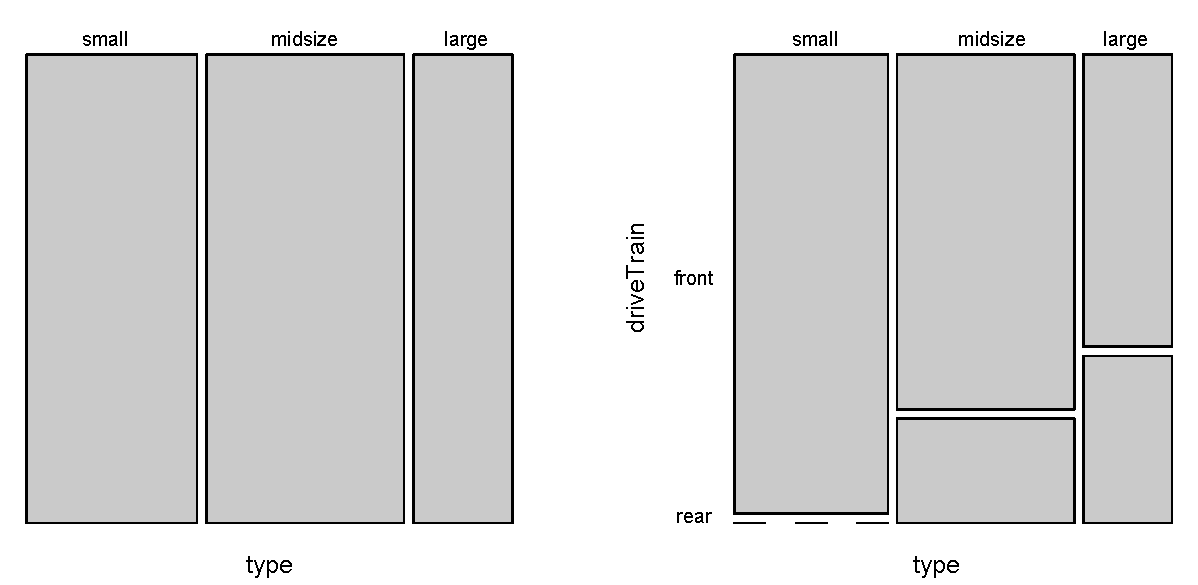
\includegraphics[height=2.2in]{01/figures/typeDriveTrainMosaicPlot/typeDriveTrainMosaicPlot}
   \caption{The one-variable mosaic plot for \var{type} and the two-variable mosaic plot for both \var{type} and \var{driveTrain}.}
   \label{typeDriveTrainMosaicPlot}
\end{figure}

The left panel of Figure~\ref{typeDriveTrainMosaicPlot} shows a mosaic plot for the \var{type} variable. Each column represents a level of \var{type}, and the column widths corresponds to the proportion of cars of each type. For instance, there are fewer small cars than midsize cars, so the small car column is slimmer.

This plot is further broken into pieces in the right panel using the \var{driveTrain} variable. Each column is split proportionally according to the drivetrain of the vehicles of that particular type. For example, the first column representing only small cars was broken into small cars with front and rear drivetrains. %In the right of Table~\ref{typeDriveTrainTableTotalsMinus4wd}, the proportion of each \var{driveTrain} level was computed within \resp{small}, \resp{midsize}, and \resp{large} cars separately. Similarly, we break apart each of the columns in the left panel of Figure~\ref{typeDriveTrainMosaicPlot} into cars with \resp{front} and \resp{rear} drive trains, which results in the right panel.
As another example, the top of the middle column represents {midsize} cars with front wheel drive, and the lower part of the middle column represents {midsize} cars with rear wheel drive. Because each column is broken apart in very different places, this suggests the proportion of vehicles with front wheel drive differs with vehicle \var{type}. That is, \var{driveTrain} and \var{type} show some connection and are therefore associated.

In a similar way, a mosaic plot representing column proportions of Table~\ref{typeDriveTrainTableTotals} can be constructed, which is shown in Figure~\ref{driveTrainTypeMosaicPlot}.

%\begin{exercise}
%What does the mosaic plot on the right of Figure~\ref{typeDriveTrainMosaicPlot} suggest about how a vehicle's \var{type} and \var{driveTrain} are related? Answer in the footnote\footnote{It appears that the larger the vehicle, the more likely it is to have a rear drive train. Do you think this result (that larger vehicles are more likely to have rear drive trains) means a vehicle being larger \emph{causes} the vehicle to have rear wheel drive? This question will be answered in Section~\ref{experiments}.}.
%\end{exercise}

\begin{figure}
   \centering
   \includegraphics[height=2.2in]{01/figures/driveTrainTypeMosaicPlot/driveTrainTypeMosaicPlot}
   \caption{Mosaic plot where type is broken up within the drivetrain.}
   \label{driveTrainTypeMosaicPlot}
\end{figure}

\begin{exercise}
Why is it that the combination \resp{rear}-\resp{small} does not have an actual rectangle? Hint in the footnote\footnote{How many cars have this combination in Table~\ref{typeDriveTrainTableTotalsMinus4wd}?}.
\end{exercise}

\begin{exercise}
Describe how the mosaic plot shown in Figure~\ref{driveTrainTypeMosaicPlot} was constructed. Answer in the footnote\footnote{First, the cars were split up by \var{driveTrain} into two groups represented by the columns. Then the \var{type} variable splits each of these columns into the levels of \var{type}.}.
\end{exercise}


%For instance, the table of row proportions is summarized by the left \term{mosaic plot} of Figure~\ref{typeDriveTrainMosaicPlot}.  This is a one-variable mosaic plot (not quite as useful as a bar plot for a single variable) then has its rectangles each split according to the second variable, \var{driveTrain}. For instance, the  en each level of \var{type} is split up by each level of \var{driveTrain}.

% The area of each rectangle in a mosaic plot is equal to the number of observations that fall in that grouping. For example, the rectangle \resp{front}-\resp{large} (the upper right rectangle) represents the cars with this combination, which is smaller than the number of


